\chapter{学习生活}
\section{工学院培养方案}
探索过工学院官网的同学可能会发现，工学院近几年的培养方案几乎是一年一改，辅修双学位的政策也时有变动。笔者认为，这与2019年开设机器人工程专业、2020年录取强基计划的学生、近年来学院课程开设情况、同学诉求等诸多因素有密切关系。

\begin{figure}[htbp]
  \centering
	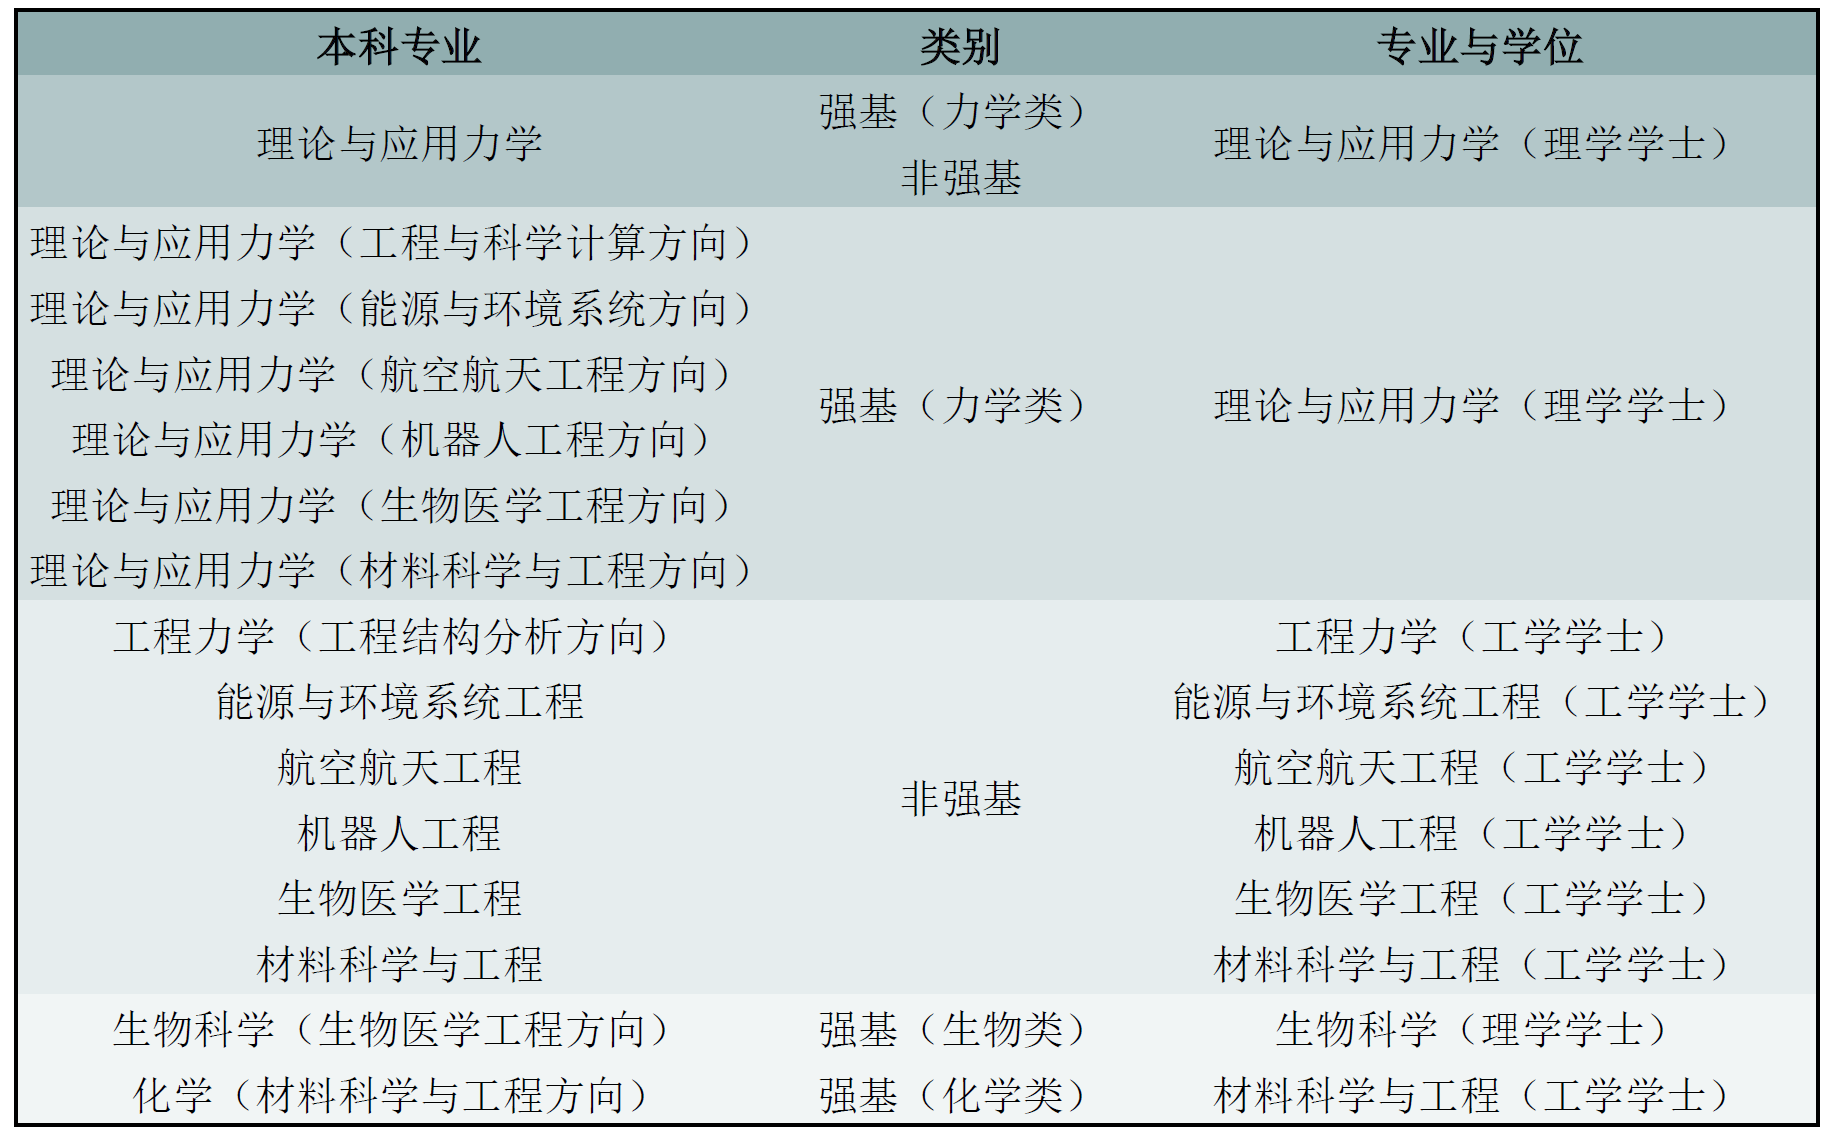
\includegraphics[width=1\linewidth]{assets/培养方案.png}
	\renewcommand{\figurename}{图}
	\caption{2024版培养方案专业情况}
	\label{fig:enter-label}
\end{figure}

\vspace{10pt}

数百位思想意识独立、成长环境各异、未来规划多种多样的本科生，若全部严格遵循一份名为“培养方案”的小册子中的表格与条款，必然导致毁灭性的结果。正如一位厨师为一千人炒一大锅菜，我敢说我夹到的那部分大概率不是夹生就是糊掉。

\vspace{10pt}

因此，阅读培养方案时，大家应时刻主动思考：我希望培养自己的哪些能力？培养方案能在哪些方面帮助我？学院暂时帮不到的方面我该如何自己找办法？希望大家辩证看待课程安排，逐渐学会分析培养方案现存的不足，取其精华，去其糟粕。

\vspace{10pt}

笔者分享自己的一些见解供大家参考。在理论学科领域一直以来的优势地位，使得北京大学在新工科发展上选择了“以科学促工程”的思路，这一思路也直接反应在了工学院的培养方案上：重视理论教学，而实践、设计、研发、创造类的培养较少。显然，工学院培养方案给予同学们最大的优势就是坚实的数理基础——各类注重理论的专业课为大家建构学科知识体系，同时在学习过程中包含了不少练习和考试。因此，认真学下来，大家会收获极为宝贵的逻辑分析能力。以数学分析为例，其本身就蕴含长逻辑链条的知识脉络，很多推导和证明也都是环环相扣；物理类课程可以训练大家的建模能力，将现实生活中的复杂问题简化抽象为可以解决的数学模型。这些能力会让我们在之后的学习和研究中更有条理、更加深入地考虑问题。

\vspace{10pt}

现行培养方案亦有难以避免的核心问题：内容难度和抽象程度较高，课程数量较多。

\vspace{10pt}

一方面，大家容易停留在抽象层面上沾沾自喜，忽视了抽象的理论知识和具体的现实问题大相径庭。如果只掌握抽象的知识，或者一些近乎炫技的解题手段\footnote{除了得分，解题手段在大学没有任何价值可言，而分数在你毕业后只是一串数字}，却不注重实际应用，那么抽象理论对于大家则毫无价值可言。这种在实例中应用的训练恐怕需要通过实实在在的大作业和科研训练来完成。对于前者，部分老师的课程含有大作业，大家可在树洞上善用搜索，在选课时予以关注考量；对于后者，大家可以通过本科生科研\footnote{一般在大二开始，少数同学会在大一下学期开始}锻炼自己。

\vspace{10pt}

另一方面，我们不可忽视时间成本。难度较高、数量较多的理论课程，想要学好、学透它们，是需要相当多的时间的。现在的大环境下，本科生进行科研训练，对于升学和选择研究生导师都是十分重要的。缺乏类似训练，势必会对后两者造成影响。而课程的难度和数量，在某种程度上对于大家及时进入科研训练是一种阻碍。

\vspace{10pt}

总而言之，工学院培养方案正在不断迭代中逐渐改进，但问题总归会有。方案本身只是一碗最为基础的大锅饭，加上什么样的菜拌着吃，是大家接下来需要认真辨析和思考的地方。

\section{基础课程}
\textbf{强调：}

以下内容为编写团队一己之见，具有一定参考价值。但我们也鼓励大家去别处，如认识的老师、学长学姐以及树洞等，寻求解答。希望大家兼听则明，敢闯敢试，探索出一条适合自己的学习之路！

\vspace{10pt}

我们还要提醒大家：学会探索属于自己的学习方法。到大一下学期，大家应该尝试着摸索，如何从了解到学好一门课程。同时切忌平时偷懒——习以为常的不了了之会导致后面越来越听不懂，引发“雪崩效应”。

\subsection{数学课程}
\textbf{1. 数学分析（一）（或：高等数学（I））}

数学分析，是一门以微分、积分为核心而展开的一系列强调“逻辑”“精确”的分析式课程。教材推荐张筑生老师的《数学分析新讲》\footnote{亦称其为“黄皮书”}，网课推荐b站上史一蓬老师的数学分析公开课。

\vspace{10pt}

笔者对于学好数学分析（一）的建议如下：

\vspace{10pt}

（1）注重“极限”“连续”“可导”“可积”等基本概念的书写，“中值定理”“泰勒公式”等定理公式的使用条件。解答习题时力求完整、严谨书写，拒绝伪证。事实上，能敏锐地发现伪证的漏洞，说明你对于概念和定理的掌握已经非常牢靠了。因此，我们建议考前进行一些有关基本概念和定理公式的系统整理记忆。

\vspace{10pt}

（2）证明题没有思路时可以尝试结合图像或题目条件进行思考，搭建大致思路后再用严谨的语言（如$\varepsilon-\delta$语言）书写。切忌一蹴而就，这样往往会导致思路混乱、漏洞百出。

\vspace{10pt}

（3）无需完全掌握一些过于复杂的证明，只需知晓大概思路即可。事实上，考试一般不会涉及这类高难度的证明，而很多新生容易在这上面花太多时间，导致整体逻辑框架混乱，重点偏移。

\vspace{10pt}

（4）鉴于数学分析极易因“想当然”而出错，掌握若干经典且基本的“反例”显得尤为重要。

\vspace{10pt}

（5）利用好习题课，多和老师、助教、同学探讨交流，互相体会对方证明或解题过程的优点和不足\footnote{也有可能发现对方是伪证（doge}。

\vspace{10pt}

\textbf{2. 数学分析（二）（或：高等数学（II））}

进入大一下学期，数学课程难度会陡然上升，你会觉得“上学期学得这么简单，但我竟然还喊不会！”这其实说明，你的水平上涨了许多。事实上，当你在学习某一课程中，感觉过程不快但又并不至于崩溃时，往往是水平上涨最快的时候。不必担心，时间会证明一切。

\vspace{10pt}

数学分析（二）会逐步介绍广义积分、多元微分，多元积分。内容看似简单，实则丰富且变化多端，尤其是多元微积分部分。因此，我们建议课前适当预习，否则容易上课走神导致整节课跟不上\footnote{笔者曾不幸体会，简直是巨大的灾难}；同时，课后认真总结和完成习题。此外，我们需要强调史一蓬老师的教学思想之一：问题不过夜。考虑到数学类课程具有极强的前后关联性，未及时解决的问题积累下来会导致后续内容学得云里雾里。因此，请大家尽量做到“今日事，今日毕”，或者至少“本周事，本周毕”。

\vspace{10pt}

具体学习建议和数学分析（一）大致相同，建议投入更多的时间和精力，适当增加练习量。

\vspace{10pt}

\textbf{3. 线性代数与几何} 

线性代数与几何，是一门介绍矩阵与行列式运算、线性变换、向量与几何为核心的课程，在多数人眼中，难度高于数学分析（一）。教材推荐David.C.Lay的《线性代数及其应用》（Linear Algebra and Its Applications），上手容易，框架清晰，70\%习题很简单，且很多题目里暗藏玄机\footnote{指暗含很多高等代数的知识，极具启发性}。如能读完本书，必定收获颇丰。

\vspace{10pt}

笔者对于学好线性代数的建议如下：

\vspace{10pt}

（1）构建思维导图，知道若干概念对应若干性质\footnote{例如“可逆矩阵定理”的24种表述}，便于后期融会贯通。

\vspace{10pt}

（2）认真完成作业，力求算得又快又对，在作业中总结方法技巧。核心知识往往只能在实际操作即做题中掌握。

\vspace{10pt}

（3）掌握基本定理的证明，因为证明中的思想和技巧能帮你更深入了解定理的来龙去脉，而且很容易用在具体的题目当中。

\vspace{10pt}

（4）多交流多探讨。线性代数往往会在周末开设“学业辅导课”，由高年级学长学姐或课程助教讲授，基础与拓展均有涉及。如有兴趣，可以一试，以进一步夯实数理基础。

\vspace{10pt}

\textbf{4. 高等代数}

如果你把线性代数学得特别通透，那么高等代数大概率不在话下。高等代数的核心知识和线性代数基本一样，会额外增添多项式理论、线性空间和空间上的线性变换、若尔当标准型等重要内容。教材推荐丘维声老师的《高等代数》\footnote{数院所用教材，部分章节无需掌握。至于是哪一部分，见仁见智，请听好老师的安排与学长学姐的建议}。

\vspace{10pt}

笔者对于学好高等代数的建议如下：

\vspace{10pt}

（1）敢于去繁从简。很多证明思路繁杂，技巧性强，没精力也没必要掌握。但是同样地，你应该知道它的核心思路；亦不可忽略包括但不限于老师所强调的、地位关键的证明。

\vspace{10pt}

（2）多角度理解一个定理到底在说什么，换而言之，把知识串起来。例如：限制线性变换和矩阵对角化的联系、最小多项式的多种求法等。

\vspace{10pt}

（3）多做题但不盲目做题。计算是工院人最基本且核心的技能。因此，我们需要掌握各种跟“算”有关的思想方法和技巧，在此基础上再去掌握证明（也会相应地变简单一些）。

\vspace{10pt}

\subsection{物理课程}
\textbf{1. 普通物理（I）}

普通物理是大家正式接触的第一门物理类课程，开课时间为大一下学期。普通物理（I）包含力学、电磁学的大部分基础内容，且两者往往以期中考试为界限分开。教材推荐钟锡华老师、陈熙谋老师的《大学物理通用教程》。

\vspace{10pt}

对于有一定物理竞赛经历的同学而言，普通物理课程几乎所有内容都是“已学习”状态。因此，笔者推荐《物理学难题集萃》（舒幼生、胡望雨、陈秉乾）作为拓展材料。

\vspace{10pt}

笔者对于学好普通物理（一）的建议如下：

\vspace{10pt}

（1）熟练掌握教材中的基本概念和经典模型，熟练程度决定解题速度上限。

\vspace{10pt}

（2）先自行完成习题，再看答案。期中或期末考试的部分题目来源于作业和往年题，平时直接照抄的一时之快，最终只会化作考场上的抓耳挠腮，得不偿失。

\vspace{10pt}

（3）进行适当拓展。受限于课时和班级人数，普通物理课程难度中等，所讲授的内容存在一些不够深入的地方，等待大家通过阅读进阶材料\footnote{老师可能会在课上列出进阶教材等。若没有，请善用搜索}等方式自行探索，构建更为完善的知识体系。

\vspace{10pt}

\textbf{2. 普通物理（II）}

开课时间为大二上学期，介绍热学、光学和近代物理三部分内容。教材仍为《大学物理通用教程》，不同老师授课进度和内容选取不尽相同。

\vspace{10pt}

笔者认为，相比普物（I），普物（II）内容更多、更注重理解，因此给出下列学习建议供大家参考：

\vspace{10pt}

（1）阅读教材多多益善，理解物理概念和物理过程。有余力可参阅其他教材，相得益彰。

\vspace{10pt}

（2）反复推导重要公式、结论，直至没有疑点。这能在解题时帮你节省相当一部分时间。

\vspace{10pt}

（3）抓大放小，关注主干内容。同样地，受限于课时等因素，教材中存在众多介绍类内容，且该部分内容在后继物理课程（如热力学与统计物理、电动力学、量子力学、固体物理等）中有严密的理论推导来支撑，所以不必事无巨细地搞清楚每一句话。

\vspace{10pt}

此外，对于普通物理课程，同一课程号的不同班级可互相替代。因此，我们建议大家选课前通过各个渠道，广泛参考不同班级的课程评价，了解工院班与数院班、地空班等不同班级、不同老师的课程侧重和授课风格，选择最适合自己的班级。当然，学有余力、力求进阶的同学可以选修物理学院开设的力学、电磁学、热学、光学、近代物理等替代普通物理。详情请咨询教务老师或参阅培养方案。

\subsection{化学课程}

\textbf{1. 普通化学B}

来到大学，化学课依旧保持了其庞杂、缺乏系统规律的特点。其主要内容是更加深入地讨论很多高中时期悬而未决的问题，比如吉布斯自由能的来源、平衡常数表达式的导出、物质的内部结构等，但难度、知识含量远远大于高中时期。教材推荐北大出版社的《普通化学原理》（蓝皮书）。笔者在此给出下列学习建议，供大家参考：

\vspace{10pt}

（1）搞清楚概念、定义，做到能够自己复述。大学化学中的概念可能对一些同学来说会较抽象，如成键轨道非键轨道等，这就需要同学们自己阅读课本，自己查资料，直到完全弄懂概念。厘清概念是整个化学学习的基石，务必要重视。

\vspace{10pt}

（2）仔细研究老师课堂上给出的例题，要自己独立的做出来，虽然面对复杂问题思考的过程可能很花时间，但对于能力培养和考试成绩都很有帮助。

\vspace{10pt}

（3）掌握多元化的解题方法。课堂上提到的方法尽量都要掌握，也基本都会在考试中用到。 妄图用单一的方法解决所有问题往往会使问题变得更难解决。

\vspace{10pt}

（4）各位上的化学课可能是开卷也可能是闭卷，但不能因为开卷考试就放松警惕，否则很有可能翻遍书都找不到答案。建议按照闭卷考试的要求学习和准备考试。

\subsection{生物课程}

\textbf{1. 普通生物学}

普通生物学B是一门Ⅳ类通识核心课，自24级开始被列为生物科学（生物医学工程方向）的专业课，选课时间为大一下学期。普通生物学B作为一门通识课，一般由佟向军老师或者陈丹英老师开课，其中佟老师的普生B同时是元培同学限定选修范围内的课程，作为生物医学工程同学的专业课的是陈丹英老师的普生B。这门课的教材是《陈阅增普通生物学》，不过其实看老师的PPT就足够了。

\vspace{10pt}

笔者对于普通生物学B的建议如下：

\vspace{10pt}

（1）关注往年题（这点的重要性毋庸置疑）。

\vspace{10pt}

（2）作为一门通识课，该课程的课业压力并不是特别大。大家可以妥善安排时间，例如在学期初完成论文翻译的工作，这样期末周的压力就会相对小。事实上，该思路适用于大多数通识课。

\section{公共课程}
\subsection{计算机基础课程}

计算机基础课程指计算概论和数据结构与算法两门课，分别在大一上、下开课，由信息科学技术学院的老师开课，多个学院同学合上。需注意，不同老师开设不同语言的课程，分为C语言和Python。C语言相对更底层更基础，Python相对更简洁开发效率更高。两种语言不分优劣，请大家自行选择。此外，一门计算机课程由课程本体和上机课两部分组成，大家需同时选择同一班级的上机课。

\vspace{10pt}

笔者认为计算机课程需注意两个方面：理论基础和代码能力。

\vspace{10pt}

理论基础会在笔试\footnote{一般为期末考试}中考察，具体内容包括但不限于计算机原理、网络与互联网基础、信息表示与存储、数据基础、算法思想和程序设计等。

\vspace{10pt}

代码能力会在上机考试\footnote{一般为期中考试，也可能单独考试}中考察，要求使用完全正确的逻辑和算法解决问题。笔试是基础，上机是应用，二者的关系类似于理论与实践，任一方面的欠缺都会影响课程学习，因此在学习过程中不宜偏废。

\vspace{10pt}

很多同学没有信息竞赛基础，或者从来没接触过代码，可能会担心不能适应课程。这样的担心是合情合理的，但也是不必要的。事实上，计算机课程会以0基础为参考水平进行教学，绝大部分同学无需考虑不能适应的问题。如果实在放心不下，可以提前寻找资料学习某一语言的基础语法。

\subsection{思想政治课程}
思想政治课程包含：形势与政策（形策）、军事理论（军理）、中国近现代史纲要（史纲）、思想道德与法制（思修）、习近平新时代中国特色社会主义思想概论（习概）、马克思主义基本原理（马原）、毛泽东思想和中国特色社会主义理论体系概论（毛概）、思想政治实践。

\vspace{10pt}

政治课最终分数一般由以下部分构成：平时分+论文分+考试分，其中考试分是主体，平时分具体打分方法因老师而异，但大多数政治课的大多数老师都会开设小组展示（Presentation）\footnote{简称pre}。大家在学期初进行分组并确认主题，小组内针对课程内容某一部分进行深入探讨，并进行一定时长的课堂展示。由此，政治课的主要任务是：准备小组展示、写论文、准备期末考试。

\vspace{10pt}

对于政治课的期末考试，平时功夫固然重要，但是期末复习尤其关键。由于不同老师讲课风格迥异，课程安排也不尽相同，而每门政治课考试是全校统一考试，因此考试题目不会有很强的个性。这也意味着题目可被穷举，且有很强的模板性。我们推荐大家通过各类渠道\footnote{详见本手册后续介绍}整理复习资料和往年题目，并多次背诵强化记忆。政治课的最终得分和期末复习时背诵的严格程度、完整程度是强正相关的。

\vspace{10pt}

最后，我们介绍思政实践课程。思政实践课程\footnote{详见practice.pku.edu.cn}包括“爱乐传习”“志愿服务”“社会实践”三个模块。“爱乐传习”即一二九合唱比赛；志愿服务如字面所述；社会实践指假期去往全国各地进行实地考察。对于思政实践，大家唯一需要注意的是时刻关注邮件和学工办通知，切勿错过选课时间。此外，在大一上学期结束时，大家可能会注意到，树洞的成绩查询中，思想政治实践显示P或IP。实际上，P意为Pass，IP意为In Process，大家无需担心。

\subsection{通选课程}
通选课是丰富同学视野、培养通识人才的重要途径，分为四个系列：I.人类文明及其传统；II.现代社会及其问题；III.艺术与人文；IV.数学、自然与技术。每个系列均包含通识教育核心课、通选课两部分课程，具体课程列表参见《北京大学本科生选课手册》。

\vspace{10pt}

通识课修读总学分为12学分，具体要求包括：

·至少修读一门“通识教育核心课”（任一系列即可）；

·每个课程系列至少修读2学分（通识核心课和通选课均可）；

·原则上不允许以专业课替代通识教育课程学分；

·本院系开设的通识教育课程不计入学生毕业所需的通识教育课程学分；

·建议合理分配修读时间，每学期修读一门课程。

\vspace{10pt}

不可否认的是，北大存在所谓“给分好”或“给分差”的通识课。但分数本身不是同学们追求的终极目标，修读通识课的意义也远不止功利层面的成绩优劣。因此，在充分参考课程测评、关注所谓热门课程之外，我们更希望大家找到、发展自己的兴趣与热爱，通过对应的通识课程开拓眼界、丰富视野，追寻心中所向。这是北大给予每位同学的宝贵机遇，我们应当好好珍惜。

\subsection{英语课程}
所有新生（英语专业学生和留学生除外）须参加英语分级考试，根据考试成绩编入A级、B级、C级和C+级，分别对应8学分、6学分、4学分和2学分的英语课程要求，并修读对应级别的课程，具体要求如下表所示。这也是培养方案中总学分是区间而非定值的原因。

\vspace{10pt}

对于在分级考试中得到C+级的同学，可进一步参加免修测试。通过测试即可获得英语免修资格。

\begin{table}[htbp]
	\centering
	
	\begin{tabular}{| l | l | l |}
		\hline
		入学分级 & 应修学分 & 应修课程类别 \\
		\hline
		A & 8 & A级课程4学分、B级课程4学分 \\
		\hline
		B & 6 & B级课程4学分、C级课程2学分 \\
		\hline
		C & 4 & C级课程4学分，或C级课程2学分、C+级课程2学分 \\
		\hline
		C$+$  & 2 & 批判性思维与学术写作\hspace{6pt} 2学分 \\
		\hline
		
	\end{tabular}
	
\end{table}

对于英语分级，我们需要提醒大家，等级高低与对应课程的趣味性、难度、选择面等没有直接关系。事实上，存在“B级相较于C级，在选择面、趣味性上更胜一筹”的声音。因此，部分同学甚至尝试“控分”以求得到B级。笔者不建议大家采取这种行为，这是对自身英语水平提升不负责任的做法。英语分级考试的目的，是通过评级大致划分每位同学英语能力的初始水平，进而应用不同的培养方案，实现英语能力的高效提升。如果通过“控分”手段得到低分，或者考前突击得到高分，评级考试就失去了原本的意义，英语素养的强化也显得捉襟见肘。因此，面对分级考试，大家不必焦虑，正常发挥，得到符合能力的评级，适应对应方案即可。

\subsection{劳动教育课程}
培养方案要求，本科阶段劳动教育学时累计不少于32学时，翻译一下，就是选一门工学院的劳动教育课程即可\footnote{至于学时到底是多少，教务会进行协调，总之选一门课就行了}。大多数劳动教育课程在暑期开课。

\vspace{10pt}

工学院目前开设五门劳动教育课：工学创新实践、金工实习、航空航天金工实习、生物医学工程金工实习、先进制造与机器人实习。请根据培养方案要求选课。例如，生物医学工程专业要求必修生物医学工程金工实习；而理论与应用力学专业并未对此作出要求，因此可以任选其一。当然，选择其他院系的劳动教育课也未尝不可，不过能否实现认定请咨询教务老师。

\vspace{10pt}

劳动教育课程以动手操作为主，旨在让大家感受工程技术在实践中的应用，体验感不错。例如，工学创新实践会以某个主题（例如无人机制作）为线索，串联起整个学期的学习，让同学们真正实现从零开始，制造作品的体验。

\subsection{公选课程，清华、北外课程}
公选课以各院系面向全校开设的课程为主，大家可自由修读这类课程。但请注意：一，根据2024版工学院培养方案，公选课不计入自主选修课学分，无法算作毕业学分；二，公选课中不仅有通识课程，还有一定比例的专业课程，请大家仔细阅读课程详细信息。总而言之，公选课和通识课一起为大家提供了一个根据兴趣选课的广阔平台，大家可以积极探索其中的好课。

\vspace{10pt}

下面向大家简要介绍清华大学、北京外国语大学的课程信息：

\vspace{10pt}

1.查阅开课名单

\vspace{10pt}

路径一：选课网——培养方案——添加其他课程——课程分类选择“公选课”——开课单位选择“教务部”——查看清华和北外的开放课程

\vspace{10pt}

路径二：北京大学教务部官网——直接搜索“清华”或“北外”——查看通知和附件

\vspace{10pt}

2.开放课程简介\footnote{在此只介绍清华课程，北外开设的小语种课程请自行利用树洞等渠道寻找信息}

\vspace{10pt}

清华向我们开放的课程，以基础工业训练中心开设的工程实践类课程为主，如制造工程体验、现代加工技术与实践等。大家可通过这类课程学习一些工程上的基本操作，小组合作完成一些作品。课程质量见仁见智。以笔者经历来看，训练中心开设课程质量总体不错。个人认为，工学院低年级同学可以选修训练中心的课程来补充实践方面的基本知识。其他院系（如航天航空学院、行健书院等）开设的课程，大家可以根据自己的需求和兴趣进行选择，在学院允许情况下可转为专业课学分。

\vspace{10pt}

3.选课注意事项

\vspace{10pt}

清华、北外课程一般比普通课程更晚录入选课系统，且选课名额较少。选课后，请务必关注教务邮件，并根据邮件内容进行进一步操作，包括清华课程网注册、掌握入校方式等。

\vspace{10pt}

值得注意的是，清华、北外与北大在作息时间上相去甚远，请大家选课时关注“备注”一栏的实际上课时间，务必预留足够的通勤时间。举个例子：北大某课程时间为8:00$\sim$9:50，清华某课程时间为9:50$\sim$12:15。此时，两校课程看似没有时间冲突，但实际上不可能及时赶到清华教室。很抱歉，我们暂未找到在两校教学楼之间瞬移的方法。一般而言，在导航软件预估用时的基础上再加5分钟，是较为保险的策略。

\vspace{10pt}

4.学分与成绩互认

\vspace{10pt}

外校课程结课后，课程成绩待下一学期开学时由教务部发邮件告知\footnote{毕业年级除外}，同时告知转学分的方式。开放课程学分可以转为本校的通选学分、全校任选学分或专业课学分\footnote{详见当年教务部官网通知，亦可和院系教务沟通确认}。清华课为等级制，不计入绩点，但是等级会出现在成绩单上。此外，转学分需要自己办理，并非默认操作。当某一门课程学分未转换时，成绩单上不会出现该课程。

\vspace{10pt}

在开放课程学习之外，笔者也推荐大家在休闲时刻，前往包括但不限于清华大学在内的其他高校，体验不同的校园风格、自然风光和人文气息。逛逛校园锻炼身体，看看风景放松身心，会会同学增进感情——即使抛开这些不谈，在清华大学入校政策日益收紧、普通游客必须抽签入校的当下，北大学子轻易放过畅通清华的机会，实在有些可惜。

\section{转入/转出工学院}
“思想自由，兼容并包”，这是北京大学一直以来的办学理念。因此，在必要的基本规则下，北京大学为大家提供了自由且多元的、寻求更佳自我发展的机会。这点很好地体现在了转专业政策上。我们必须认识到，任何院校的任何转专业政策，都不可能没有任何规则和限制，否则全校几千人都跑去通班\footnote{隶属于元培学院}学当下最火的人工智能了！北大亦是如此——存在一系列考核选拔、强基计划转专业范围受限\footnote{详见本手册1.2节}等。笔者必须强调的是，转专业存在一定门槛，转入某些院系可能面临很强的竞争，请大家慎重考量，在转专业前做好脑力和心理双重准备。

\vspace{10pt}

获取转专业信息的主要途径有：

·北京大学教务部官网-“学籍异动”页面

·春季学期开学初全校范围内组织的转系/辅双经验介绍讲座（自行关注相关通知）

·拟转入院系官网、公众号

·有相关经历经验的学长学姐

·北大树洞

\vspace{10pt}

下图为工学院本科生转出情况及转入情况\footnote{数据可能有±1误差}：
\begin{figure}[htbp]
	\centering
	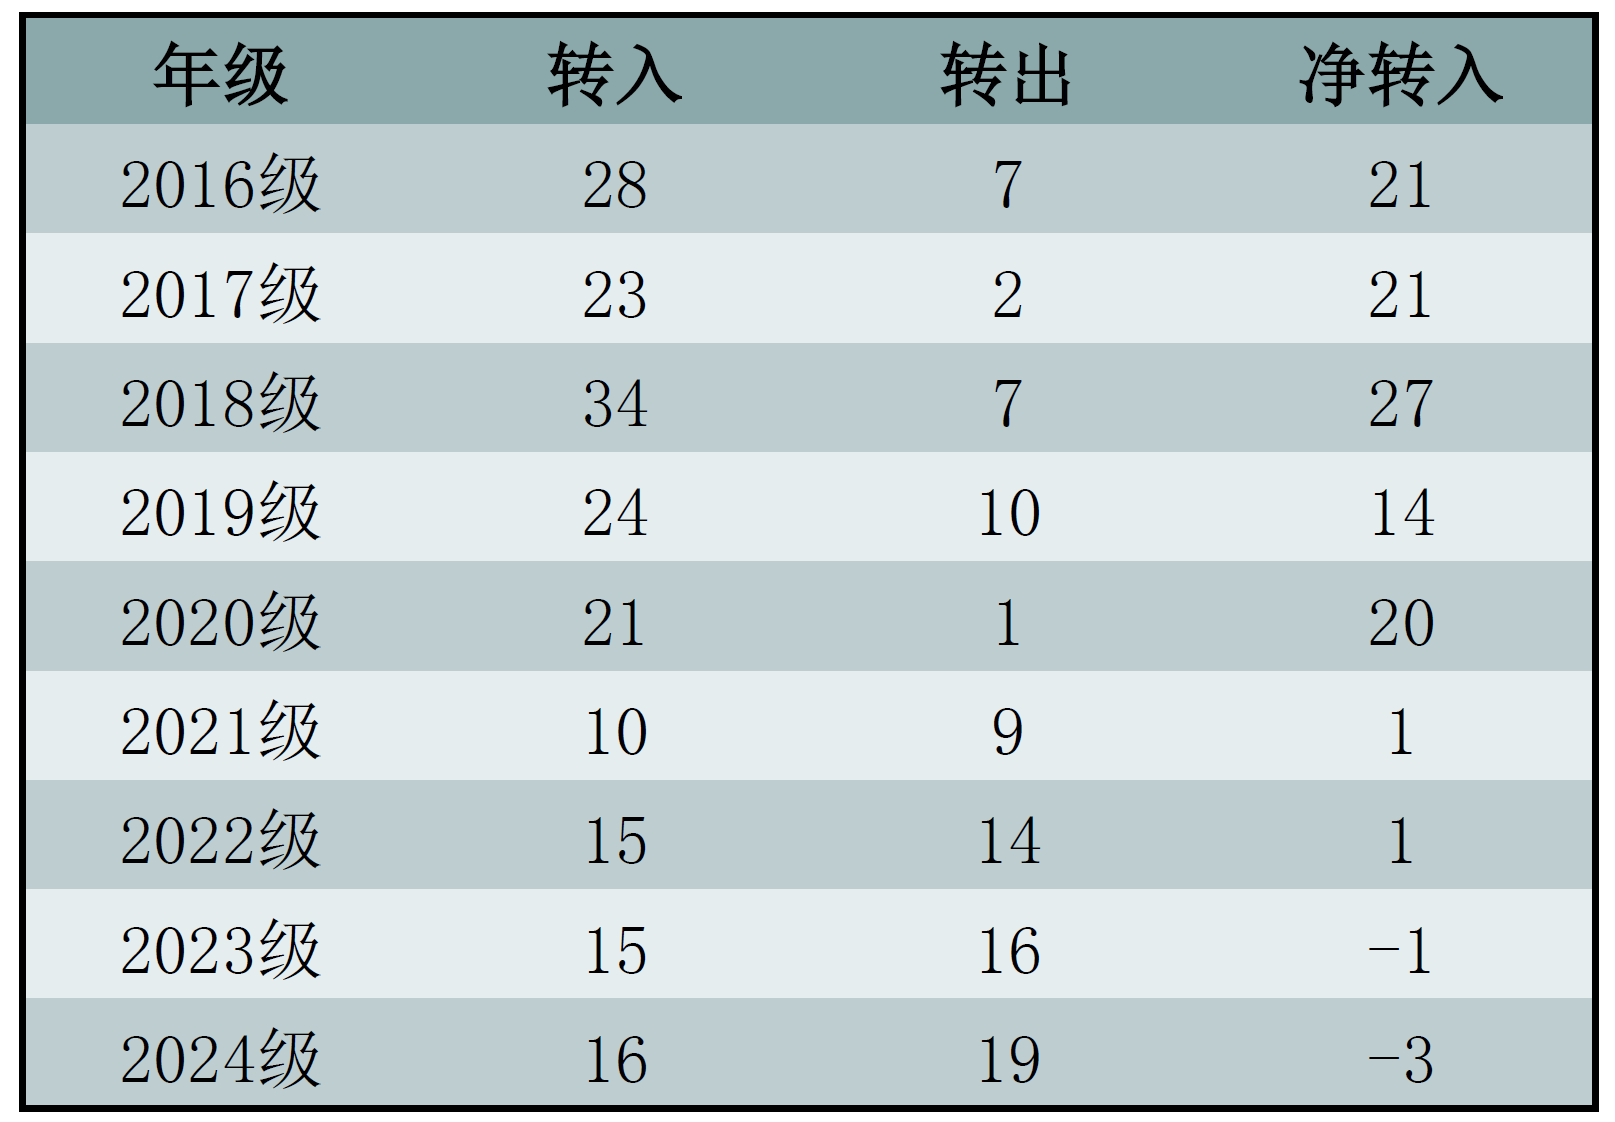
\includegraphics[width=0.6\linewidth]{assets/转入转出情况.png}
	\renewcommand{\figurename}{图}
	\caption{工学院本科生转入转出情况}
	\label{fig:enter-label}
\end{figure}

在这里，我们也为大家找到了几位智慧而热心的学长学姐，分享他们有关自己成功转专业的经历经验。

\subsection{工学院转出经验分享}
\subsubsection{（1）工院$\to$信科$\parallel$作者：一位希望保持匿名的同学，大一平转转入信科信息与计算科学专业（智班）}

\textbf{转院考量}：兴趣，以及对于未来的规划。建议入学后多了解各个方向，形成更全面的认识后再做决定。本人转信科并非因为觉得工院不好，而是心中向来对计算机抱有更大的热忱，报考北大时就已经坚定地向往去信科学习，只不过因为种种原因被调剂至工院。

\vspace{10pt}

\textbf{转院流程}：每年报名及考试时间不尽相同，请密切关注院系相关通知，或民间的转信科微信群。大概在每年三四月份，信科发布转院系通知后，按照要求填写和提交相关材料。之后教务会通过邮件通知考试时间和安排，按要求参加考试即可。

\vspace{10pt}

\textbf{课程规划}：仔细比对信科和工院（自己预期方向的）培养方案，做好转入信科和留在工院的两手准备。大一上的课大体相似，但是信科上计算概论A，工院上计算概论B（根据以往经验，如果计算概论B上80分，可以不用重新修读计算概论A）；工院上自己开设的数学分析和线性代数/高等代数，信科上数院开设的相应课程（根据以往经验，可以替代）。【以下仅针对部分计算机相关方向的专业，其他例如电子信息等专业会略有不同】大一下的课有部分差别。根据以往经验，普通物理Ⅰ可以替代专业选修课的物理类课程。信科多出来的两门专业课\footnote{程序设计实习和人工智能引论}需要在之后补修，可以选择这其中一门时间不冲突的专业课，减轻之后的补课压力。数据结构与算法B不可替代数据结构与算法A的，且数据结构与算法A是在秋季学期开课。

\vspace{10pt}

\textbf{考前准备}：多刷题，打好基础即可。转计算机相关专业的是机考（算法题），转电子信息相关专业的是笔试（物理）。民间转信科微信群里可能会有往年题，可以参考。面试中规中矩，不过也可以稍微准备一下。

\vspace{10pt}

\textbf{住宿调整}：一般不会换寝室。若确有需求，可自行找宿管申请。

\vspace{10pt}

\textbf{心态调整}：放平心态，即使没考过，大二还有机会，虽然届时课程规划会比较麻烦。实在没考过也不必太沮丧，工院也是非常值得留下来的。俗话说，三百六十行，行行出状元，真的用心学的话，在哪儿不都一样？

\subsubsection{（2）工院$\to$数院$\parallel$作者：原2022级\ 秦晟，大一降转转入数院数学与应用数学专业}
对于转院，我认为问题最大的可能不是报名流程，而是自己为什么要下这个决定。

\vspace{10pt}

1. 首先掂量的是自己想法的“纯度”和“目的性”。一定要避免一时脑子热、跟大流等类似情况。可以旁听几节课，并且注重自己在学这些课程的内心体验，看看是否真如自己所想。

\vspace{10pt}

2. 关于摇摆不定，我十分鼓励大家在遇到可能包括转院在内的各种疑惑时，多和老师、家人、同学沟通，之后再看看自己的想法是否有所松动。

\vspace{10pt}

3. 关于平转降转，仁者见仁，智者见智。一年的时间，可以看作节省，也可看作积淀。不同的选择有不同的注意事项：平转，提前选课；降转，较为灵活。

\vspace{10pt}

4. 关于流程，教务部每年都于四月中旬发布校本部转专业工作通知与各院系接收人数和考核计划，学生会也会组织转专业、双专业、辅修的交流会，有意向的同学可以关注北大教务部和校学生会公众号。

\vspace{10pt}

5. 关于重视程度，大家可能会将这类事情看得很重，认为大学专业关系到人生职业、未来发展，就犹豫不觉、不知所措。我想说的是，这么想百分之百没问题，但人生纷杂难测，机会众多，遵循当下自己的真实内心想法就好。

\vspace{10pt}

祝大家大学本科4（or 5 or 6）年快乐。

\subsection{转入工学院经验分享}

工学院的各位同学大概率用不到这部分内容，但是如果你身边有对转入工学院有兴趣的同学、朋友，可以把这些内容推荐给ta！

\subsubsection{（1）物院$\to$工院$\parallel$作者：2023级\ 李宗远，大一平转转入工学院机器人专业}

北大在大一下和大二下分别有一次转专业机会。我这届转专业在四月初开始报名，报名方式参考北大公示的文件。不过每年时间可能不一样，大家及时关注学院官网上发布的信息以及邮件。至于考核和接收时间就是各个学院自行决定了。我这届是在5月15日进行面试，大概一周后工学院公示转专业结果。

\vspace{10pt}

每年都北大会发布《XX年校本部各院系转院（系）转专业接收工作具体方案》，内含各个学院所接收的转专业人数、报名条件、报名方式以及考量方式等。在学院官网中可以找到以往的文件。2023和2024年工学院的报名条件都是“在校期间无不及格课程”，听往届学长说以前还对绩点有要求。

\vspace{10pt}

23年与24年工学院的转入考量都只有面试。我这届的面试流程是：学生先进行一分钟的自我介绍（随便说说就行，没多少影响），然后是老师提问。对我而言，老师问的问题是“你这学期选了多少学分的课”“你这学期选的专业课期中考试考了多少分”，然后提醒我要提高自己的绩点，我的面试就结束了（狗头）。我的面试时间属于很短的，我个人推测是因为我大一所修的课程和工院的培养方案基本吻合，并且我大一下的几门专业课的期中成绩都不错。

\vspace{10pt}

老师面试的主要目的是了解学生的情况，未必会问具体的专业问题。大多数老师也都很和善，现场的氛围倒是和茶话会挺像。和我一起参加面试另一位同学就被面试了五六分钟。他是一名大二的学生，想要降转工院。但他学习的数学课程是C级，而且在疫情期间选过pf，也退过课。我说的这三条都是面试过程中老师问他的点。

\vspace{10pt}

23年工院的招收人数是30人，最后公示接收人数是二十几人。24年工院的招收人数是40人，报名人数21人，接受人数16人，其中选择机器人工程的占了一半。在报名人数仅占接受人数一半的情况下，还是刷掉了五个人。个人推测，他们被刷掉的原因可能如下：课程选择与工院培养方案大相径庭或者成绩不好，工院老师担心他转入后跟不上课程进度；还有一种可能是选择转入机器人专业的人太多了，工院老师要考虑机器人系学生的保研竞争问题。

\vspace{10pt}

至于平转和降转，大家可以根据自己情况来选择，如果像我一样大一选的课和工院培养方案基本吻合，就可以选择平转，如果专业课有很大不同也可以选择降转，这样可以较好的跟上课程进度。如果课程相差很大还选择了平转，面试老师有可能会问你能不能跟上课程之类的问题。

\vspace{10pt}

如果以后工院的转专业考核还和24年一样的话，我的建议是在平时用功夫，多修些相关专业课，把成绩拉高，有什么问题及时询问工院的教务老师和有相关经验的学长学姐。也要记得去官网找最新的我在上文中提到的那几个文件——在大学里信息搜集能力十分重要。至于面试，没多少好准备的。当然，如果考核方式有所变化，就不要按照我的建议来啦。

\textbf{课程规划：}

在前文我也提到，我大一的课程选择与工院的培养方案基本吻合，这在一定程度上帮助我顺利通过工院的面试。因此，同学们可以去北大官网了解本科生培养方案（要找最新版的）。如果在大一上开始前或大一下开始前就决定转入工院的话，可以按照工院的培养方案进行选课，这样转过来以后就不用再补课了。或者选一些可以平替工院的课，比如B级及以上数学课。例如，工院23年的培养方案上写着，非强基生可以用高数B代替工院的数学分析。其实理学部学生大一的专业课有很多相似之处，比如高数，线代，普物，计概和数算，无非是不同专业难度不同。所以理学部的学生转入工院还是比较轻松的，如果是文科的同学想要转入工院，我建议提前修一些相关的专业课。

\vspace{10pt}

非工院学生要在选课的第三阶段才能选工院的专业课，不过工院大一的课程容纳人数很多，名额有很多空余，基本不用抢，在第三阶段选课也没什么影响。

\textbf{住宿调整：}

同学们在转完专业后，可自行选择留在原宿舍或申请换宿舍。留在原宿舍的好处是，和舍友已经很熟了，不用再磨合。如果和原宿舍同学相处得不太愉快，也可以借此机会换一个宿舍。新宿舍的同学有可能也是工院的，大家平时还可以一起交流讨论专业问题。转宿舍的具体流程，需和原学院以及工学院的学工老师沟通。

\textbf{心态调整：}

转入工院的难度要比热门的信科、数院小一些，考核也不多。因此，同学们不必焦虑，平时认真学习别挂科，在选课上多花些心思，提前去了解工院的几个专业，确定好自己的目标，转入工院就是水到渠成的事啦。

\vspace{10pt}

最后预祝想要转入工院的同学们都成功转进自己心仪的专业，欢迎你们加入工院这个温暖的大家庭！

\subsubsection{（2）生科$\to$工院$\parallel$作者：2022级\ 王喆楷，大一降转转入工学院工程与科学计算方向}
\textbf{\textbf{关于降转和平转}}\textbf{\textbf{：}}

平转即两专业学习无缝连接，降转则需要在新专业多读一年。

\vspace{10pt}

如果大家在转专业前后课程重复度较高，或者在转专业前所修的部分专业课，经过目标院系院教务认证，可以替代本院培养方案中的课程，个人认为可以直接选择平转。毕竟大一以通识教育为主，不同专业的培养方案大相径庭，有心预习目标院系的专业课的话，适应平转的压力并不大。

\vspace{10pt}

当然，也不必视降转为逃避。如果专业跨度较大，或者关键课程没有修读，完全可以投向降转。多余的一年时间可以更好地适应大学的模式，思考自己真正需要什么。担心荒废时间的话，可以在学有余力且确有热爱的情况下攻读一门双学位，或者提前联系导师进组。（P.S. 亲身体验，唯一的尴尬是说出自己的年级常常伴随着怀疑的目光……）

\textbf{住宿调整：}

转专业并不意味着会安排新宿舍。据我了解，除元培PPE和光华未来领导者等少数项目中，转入/申请者均搬入了对应的住宿，其他的转专业同学大多仍然维持着原宿舍。搬到同一寝室有助于专业课学习上的互帮互助，也能更快融入新学院。不过就我自己而言，选择了维持原宿舍，因同寝室内共三人转院，算上双学位便在一间寝室内凑出了六门专业，被朋友戏称小元培（bushi），在学术探讨方面为我提供了更多的跨学科体验。

\vspace{10pt}

住宿调整方面，可以直接前往宿管中心进行询问并申请调整，没有时间限制，随时有空位即可搬。值得一提的是，对于降转的同学，即便当前不换宿舍，在原定的毕业年份时（大三结束后）也需要搬出原宿舍另择宿舍。

\vspace{10pt}

\textbf{转院流程：}

1.询问往届学长学姐，善用搜索，了解往届院系互转的具体政策。我认为应该主要聚焦于一下信息：

·目标院系对转入专业有无限制/本院是否允许转出

·是否对降转/平转有特别要求

·是否需要某门课程必修 \& 该课程成绩要求

·对于成绩要求

·考核方式（面试/笔试）及可能涉及内容

\vspace{10pt}

在我转专业的那一届，信科仅限平转，设置上机考试且要求需修过计概A；物院转院考试，大一考察力学，大二涉及四大力学；数院则大一大二共用考卷……每年具体政策不同，以上仅为参考。建议尽量掌握当年的相关信息，以便规划自己的选课方案和时间管理。

\vspace{10pt}

2.北大教务网搜索转专业专区，下载附件，了解转专业申请时间线的大致的时间节点。

\vspace{10pt}

3.开放申请后，按照要求准备手续材料。

\vspace{10pt}

4.应对考核，静待结果。

\vspace{10pt}

最后，切莫把转专业当作治愈所有问题的良方。未来规划和学科适应程度确实改变了，可是你所遇到的问题却不会烟消云散，需要你自己去面对和解决。如果因种种原因未能如愿转系，也请放平心态，在北大自由的选课制度和双专业/辅修制度下，找到你的热爱。

\newpage

\section[双专业/辅修建议]{双专业/辅修建议\footnote{根据《北京大学2025年本科双专业申请审核工作通知》，2024年（含）以后入学的本科生按照《北京大学本科生修读双专业管理办法》执行。因此，对于大家而言，“双学位”已经是过去式。更多有关双专业、双学位、辅修的区分，详见3.5.4}}

\subsection{双专业/辅修简介}
北京大学鼓励学有余力的同学修读双专业、辅修专业，成为复合型人才。

\vspace{10pt}

修读双专业或辅修专业的部分考量列举如下：

（1）对某个非主修专业方向很感兴趣，有志于深入钻研的；

（2）认为某个非主修专业方向能够提升自己今后的能力、眼界、人脉、竞争力等的；

（3）希望以后直接转行至该行业的。注意：强基计划同学跨院系保研其他专业存在一定限制，请关注最新通知；

（4）希望所学辅双专业为主修专业赋能的。例如，信息学双学位可进一步提高代码能力，便于工科学业未来发展；

（5）暂时没有明确想法，但是学有余力，希望进一步丰富大学学术生活的。

\vspace{10pt}

当然，选修双专业或辅修专业的最大挑战是课业压力。例如，工院强基理力+经济学双学位的毕业要求约190学分\footnote{每年均会有所变动，请关注最新信息}。不过，学长学姐的经验告诉我们，时间就像海绵里的水，只要愿意挤一挤还是有的（bushi）。

\vspace{10pt}

关于双学位、辅修的常见核心问题，北大教务部网站有详细解答。具体路径：北京大学教务部官网——学生——双学位/辅修。双学位、辅修的详细培养方案也可通过上述路径获取。此外，学校或各院系会在春季学期初期举办转专业/辅双经验介绍讲座，有兴趣的同学可自行关注。

\vspace{10pt}

下面列出若干双专业/辅修的注意事项。笔者再次提醒大家，本手册任何有关现行政策的内容仅作参考，手册不保证绝对的准确性和时效性，请大家务必关注学校、各学院发布的最新通知。

\vspace{10pt}

（1）双专业需正式报名；辅修无需任何手续，直接选课、上课，并在毕业时向教务申请相应专业的学位认定即可。无法继续双专业学习时，可以申请退选双专业；若达到辅修毕业要求，也可在毕业时转为辅修。

\vspace{10pt}

（2）双专业课程通过专用通道进行选课，直接抽签决定而无需投点，每学期学分上限为30学分，根据该学期双专业课程学分总和收费\footnote{以国家发展研究院的经济学双专业为例，校内本科生学费为150元/学分，教学计划共42学分，总计6300元}。辅修课程通过普通选课“跨院系选课阶段”进行投点选课，每学期上限仍为25学分，不额外收费。

\vspace{10pt}

（3）双专业毕业要求学分多于辅修要求，具体数据大约是45：30，各院系各项目存在差异，主要体现在双专业要求的专业选修课会更多。

\vspace{10pt}

（4）某一门课程的学分只可认定一次。例如，国发院开设的经济学原理（3学分），既是通识课，也是经济学双专业的必修课。因此，在毕业时，该3学分或计入主修专业的通识课学分，或计入经济学双专业的必修学分，二者任选其一而不可兼得。

\vspace{10pt}

（5）毕业证书中标注双专业。例如，工学院力学类强基生选择了生物医学工程方向，则其毕业证上的专业标注为“理论与应用力学+生物医学工程辅修”；如果该同学还修读了国发院经济学双专业，则其毕业证书上或标注“生物医学工程辅修”，或标注“经济学双专业”。

\vspace{10pt}

（6）学位证书仅有一本。原有的双学位项目可获得两本学位证书，现行的双专业项目仅可获得一本学位证书，对于双专业授予辅修学士学位\footnote{注意：通过辅修是无法获得辅修学士学位的，所以虽然名为“辅修学士学位”，实则需要通过双专业获得}，辅修学士学位在主修学士学位证书中标注。

\vspace{10pt}

（7）重要时间节点：每年春季学期初，学校、各院系会开展转专业、双专业讲座，推荐大家关注。转专业、双专业的报名工作大约在4、5月开始，请大家关注学校、各院系的官网和公众号等信息渠道，亦多多关注自己的邮箱，防止漏失重要信息。

\vspace{10pt}

（8）双专业门槛：不同院系要求各异，但共同特点是门槛几乎为零，一般而言不挂科、成绩正常就行，且一般无需考试选拔。

\vspace{10pt}

（9）部分双专业/辅修与主修专业是互斥的，即特定的A、B专业不能同时作为主修和双专业/辅修。不过，工学院在这方面几乎没有受到限制。具体互斥信息请参见《北京大学辅修/双专业与主修专业互斥一览表》

\vspace{10pt}

（10）培养方案是不断更新的，且近几年也有新的辅修或双专业项目开设，请大家以最新文件为准。

\subsection{常见问题解答}
\textbf{（1）我到底应不应该修读双专业？}

浓厚长久的兴趣是修读双专业的关键。它能提供动力，有助于学好课程，在课堂内外主动获取更多相关知识。建议同学们在修读前，对培养方案、院系氛围、讲课内容进行一些了解，例如可以旁听课程，也可以咨询学长学姐。实在无法坚持学习，也可以选择退出。这并不丢人——大学是人生中试错成本最低的阶段，敢闯敢试才能让我们的青春不留遗憾。

\vspace{10pt}

事实上，笔者想强调的是，包括是否修读双专业在内的大学学习生活中的众多决策，功利因素的占比远没有大家想象的那么大，很多时候仅需问问自己：我真正感兴趣的是什么？跟着自己的内心走，才会有长久的动力。

\vspace{10pt}

\textbf{（2）学双专业有什么实际作用？}

实话实说，最大的作用不仅在于毕业证书和学位，更在于你在课堂上真正学到了什么，玄乎一点，是学习能力的提升和个人眼界的拓展，是对大学生活的一种充实和拓展。当然，双专业也对从事对应行业有一定程度上的帮助，至于程度大小：

\begin{figure}[htbp]
	\centering
	
\includegraphics[width=0.2\linewidth]{assets/2.1.1衡量.png}
\end{figure}

\vspace{10pt}

\textbf{（3）修双学位要提前准备什么吗？}

无需刻意准备，先把主专业学好了再说。兴趣十分浓厚的同学可自行阅读相关专业书籍。

\subsection{学长学姐经验分享}
\textbf{国家发展研究院-经济学双学位$\parallel$作者：2020级\ 瞿朱毅}

经济学双学位由北京大学国家发展研究院开设，据往年经验，一般要修42学分左右，包含必修课：经济学原理、中级微观经济学、中级宏观经济学、计量经济学和中国经济专题，以及其他选修课。在各个双学位课程中，经济学双学位相对轻松，录取也较为容易。想要未来从事经济学学术科研的同学可以选择相应课程，如做微观理论的可以选学产业组织、博弈论等，如想转商科金融的建议尽早修完财务会计和财务报表分析等。

\vspace{10pt}

我当初选学经济学双学位是怀着跑路的心态去的，就是想通过修经济学双学位研究生转往经济学方向，但后来发现经济学学术科研内部内卷严重，工院给分一般导致研究生转到经济学较为困难，故放弃该想法，就把经济学纯当一个兴趣和“白月光“式的存在了。后来强基计划保研政策也公布了禁止转入经管。

\vspace{10pt}

感觉我最后还是有一些收获，譬如做了助教挣了钱，找到了女朋友（笑），也学会了用经济学的视角分析问题。当然也有遗憾啦，遗憾就是大一没有选上双学位导致有一些必修课放到了紧张的大三去修。优势就是能够多拿一个学位（笑），多认识一些人，多获得一些知识，以及提升绩点，劣势就是在大四还有一堆课，挤占了科研时间。如果说有啥建议的话，那我该说，去努力发掘自己的爱好是一件重要的事情，有些时候经双修的好能够给你从工院低分的挫折里找回信心。

\section{学业导师}

\subsection{简介}

工学院会为每位新生统一安排一位学业导师，请大家关注教务老师的通知。根据笔者经历，每位导师负责3至4位同学。每学期，大家需要和学业导师至少完成3次面谈交流，并填写指导记录，在每学期的期末周前上交至院系教务处。

\vspace{10pt}

学业导师主要关注同学的大学生活适应、选课上课、专业方向选择、个人学习计划制定、职业生涯规划等，会在力所能及的范围内，给予大家真诚的建议。鉴于许多学业导师都有自己的课题组，所以除了课业与生活，大家也可向自己的学业导师了解行业学界前沿和导师研究方向，亦可在他们的指导帮助下参观实验室、阅读相关论文等，增进自己的综合学术能力。

\subsection{一些补充}

（1）部分同学可能囿于性格内向，不愿或不敢与学业导师交流太多。事实上，大家无需紧张担心，在最为基础的礼貌之外，许多老师都是十分随和的，大家把老师们当作是一位朋友即可。不必担心“我说了这句话，老师可能会对我产生什么看法”，也无需害怕“我的这个观点和老师的不一致，会遭到强烈反对”。大学之大在于有容乃大，大家在不打破基本原则、不违反公序良俗的前提下，尽情表达自己的真实想法，相信老师一定会给予尊重和真诚的指导。

\vspace{10pt}

（2）大家在每次面谈交流结束后，需填写指导记录并交由导师签字。指导记录表可在学院教务办公室直接领取纸质版，亦可从工学院官网下载打印。

\vspace{10pt}

（3）建议大家在学期初规划面谈大致时间，例如第1、8、16周。我们推荐大家参考开学、期中考试、期末考试这三个时间点，以期与学业导师的交流带来更多收获。或许老师考前的某一句复习指导就点通了你的任督二脉呢？

\vspace{10pt}

（4）提前发送邮件，与学业导师预约具体时间。正式的格式、有礼的称呼和礼貌的问候总不会出错。建议在预约时间前5分钟左右到达\footnote{视情况而定，并非墨守成规}，这一小段时间体现的，是你对学业导师的尊重和对面谈交流的重视。

\vspace{10pt}

（5）对每次交流予以足够重视。老师们学术科研经历丰富，研究方向各异，他们的分享和指导对我们的学习方法、未来方向、生涯规划甚至价值观念，都会有一定程度的影响。因此，我们应该充分利用好学院给予我们的宝贵资源，在话语之间力求自我提升。切忌把面谈看作是被迫完成的任务，那会使指导效果大打折扣，且会令你在未来的某个时刻后悔，为何当初没有好好珍惜交流机会。
